% This file was created with tikzplotlib v0.10.1.
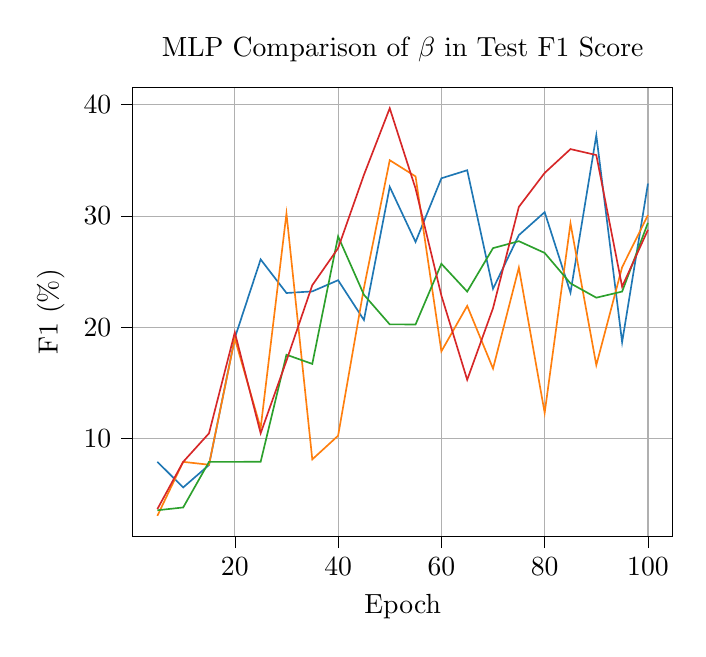
\begin{tikzpicture}

\definecolor{crimson2143940}{RGB}{214,39,40}
\definecolor{darkgray176}{RGB}{176,176,176}
\definecolor{darkorange25512714}{RGB}{255,127,14}
\definecolor{forestgreen4416044}{RGB}{44,160,44}
\definecolor{steelblue31119180}{RGB}{31,119,180}

\begin{axis}[
tick align=outside,
tick pos=left,
title={MLP Comparison of $\beta$ in Test F1 Score},
x grid style={darkgray176},
xlabel={Epoch},
xmajorgrids,
xmin=0.25, xmax=104.75,
xtick style={color=black},
y grid style={darkgray176},
ylabel={F1 (\%)},
ymajorgrids,
ymin=1.24208134217142, ymax=41.5147128108794,
ytick style={color=black}
]
\addplot [semithick, steelblue31119180]
table {%
5 7.92000792000792
10 5.62202060587421
15 7.63850450359785
20 19.0518730543616
25 26.1066971142955
30 23.0869606203889
35 23.2321220938959
40 24.2366329322851
45 20.6618401906785
50 32.6191868275793
55 27.6744532063681
60 33.3930959184643
65 34.1165645518736
70 23.4642796879143
75 28.2831605014704
80 30.3520349323678
85 23.1224881513597
90 37.2510725935087
95 18.6757405031517
100 32.9138806062151
};
\addplot [semithick, darkorange25512714]
table {%
5 3.07265549983997
10 7.92000792000792
15 7.66206270793427
20 18.9854523287807
25 10.9526101428935
30 30.2265928141939
35 8.14000814000814
40 10.2683818727961
45 23.5463029432879
50 35.0180721480745
55 33.5592057563343
60 17.8482396214652
65 21.9298265448946
70 16.2991969204221
75 25.3642051454496
80 12.3251748251748
85 29.3430262861922
90 16.6100947762839
95 25.4083817681248
100 30.0816426293496
};
\addplot [semithick, forestgreen4416044]
table {%
5 3.57142857142857
10 3.82363538101243
15 7.92000792000792
20 7.92000792000792
25 7.92584438431703
30 17.5441046111149
35 16.7186844989076
40 28.1747481231138
45 22.9294666994348
50 20.269344898425
55 20.2629494356635
60 25.7134170177648
65 23.2134137771277
70 27.1181227421409
75 27.743652359037
80 26.6886081012997
85 23.9557539273619
90 22.6672125007621
95 23.2182119779537
100 29.3911020324722
};
\addplot [semithick, crimson2143940]
table {%
5 3.67751060820368
10 7.92000792000792
15 10.4825034684754
20 19.5496810881426
25 10.4853264787506
30 17.0014657802779
35 23.7844710898473
40 27.110857711398
45 33.6992672567618
50 39.6841386532108
55 32.4687638584188
60 22.8615279970002
65 15.2902877913363
70 21.7249161586973
75 30.8221052164525
80 33.8754341376431
85 36.0150605214201
90 35.4791460365894
95 23.6560883725572
100 28.7637524103272
};
\end{axis}

\end{tikzpicture}
